\documentclass[12pt]{article}
\usepackage[margin=1in]{geometry} 
\usepackage[normalem]{ulem}
\usepackage{graphicx,amssymb,multirow,amsmath,amsthm,psfrag,setspace,subcaption,float,cite,authblk,color,url,mathtools}
\usepackage{amsxtra}
\usepackage{amsthm,amsmath,amssymb}
\usepackage{mathrsfs}
\usepackage[colorlinks=true,bookmarks=true]{hyperref}
%\usepackage{breakurl} %%This package must be after hyperref
\usepackage{float}
\usepackage{cite}
\usepackage{graphicx} 
\usepackage{listings}
\lstset{breaklines}  %让LaTeX自动将长的代码行换行排版
\usepackage{color}
\usepackage{appendix}
\definecolor{dkgreen}{rgb}{0,0.6,0}
\definecolor{gray}{rgb}{0.5,0.5,0.5}
\definecolor{mauve}{rgb}{0.58,0,0.82}
\usepackage[table,xcdraw]{xcolor}
\lstset{
  language=matlab,                % the language of the code
  basicstyle=\footnotesize,           % the size of the fonts that are used for the code
  numbers=left,                   % where to put the line-numbers
  numberstyle=\tiny\color{gray},  % the style that is used for the line-numbers
  stepnumber=1,                   % the step between two line-numbers. If it's 1, each line 
                                  % will be numbered
  numbersep=5pt,                  % how far the line-numbers are from the code
  backgroundcolor=\color{white},      % choose the background color. You must add \usepackage{color}
  showspaces=false,               % show spaces adding particular underscores
  showstringspaces=false,         % underline spaces within strings
  showtabs=false,                 % show tabs within strings adding particular underscores
  frame=single,                   % adds a frame around the code
  rulecolor=\color{black},        % if not set, the frame-color may be changed on line-breaks within not-black text (e.g. commens (green here))
  tabsize=2,                      % sets default tabsize to 2 spaces
  captionpos=b,                   % sets the caption-position to bottom
  breaklines=true,                % sets automatic line breaking
  breakatwhitespace=false,        % sets if automatic breaks should only happen at whitespace
  title=\lstname,                   % show the filename of files included with \lstinputlisting;
                                  % also try caption instead of title
  keywordstyle=\color{blue},          % keyword style
  commentstyle=\color{dkgreen},       % comment style
  stringstyle=\color{mauve},         % string literal style
  escapeinside={\%*}{*)},            % if you want to add LaTeX within your code
  morekeywords={*,...}               % if you want to add more keywords to the set
}



\numberwithin{equation}{section}


\newcommand{\mbr}{\mathbb{R}}



\begin{document}
\section{Project Title} Arduino-based experimental for the study of unsteady heat transfer temperature of metals
\section{Project Objective} 

The aim of this experiment is to investigate the rate of temperature change of a metal cylinder in unsteady heat transfer 


The metal rod is between two heat sources, and to investigate the relationship between the experimental hypothesis and the temperature of the heat source, its position in metal, length, material and other factors. 


The completion of this experiment will contribute to the study and understanding of unsteady state heat transfer.



\section{Hypotheses}

\begin{enumerate}
  \item Before reaching the steady state, the rate of temperature change at the point becomes faster with the enhancement of thermal conductivity of the material.
  \item Before reaching a steady state, the rate of temperature change at the point becomes faster with the shortening of the metal length.
  \item Before reaching the steady state, the rate of temperature change at the point becomes faster with the increase of heat source temperature difference.
\end{enumerate}

\section{Methodology}
The experiments were carried out using two materials(Iron and Aluminum), a combination of length variation(250mm \& 250mm*2), temperature variation by adjusting the temperature of the domestic kettle, and ten sensors set at different locations to collect the temperature variation at different distances. More information in Methodology.


The experiments will focus on these variables, while using the data generated to obtain additional phenomena and conclusions beyond the hypothesis, in order to investigate the variation of temperature in the heat transfer of metals in a non-stationary state.


















\subsection{Real Experiment Methodology}

In this experiment, we use 250mm 10mm diameter carbon steel bar and 250mm 10mm diameter pure aluminum bar as the experimental objects. We install the test sample at about 25cm above the desktop through our designed 3D printing parts, so that it can be fully placed in contact with other objects. On both sides of the polished smooth sample, we close it to the copper sheet soaked in water for a long time as the heat source.


We use Arduino's hardware platform as the data collector, and use MATLAB software to monitor and process the recorded data in real time. We use DS18B20 sensor as our temperature sensor, install it in the 3D printing part, and make it fully in thermal contact with the point to be measured. At the same time, We put two waterproof temperature sensors into cold and hot water at both ends. This will be used to monitor the heat source and prevent the failure of the experiment due to possible unstable factors of the heat source.
%TODO 这里插入图片

The real experiment will be completed within 2 weeks after the mid-term examination. At that time, the data can be collected and analyzed.



\subsubsection{Instrument Detailed}
These are the main metal parts used in our experiment,Stick \ref{Stick} and Sheet \ref{Sheet} which are purchased off the shelf.

\begin{figure}[htbp]
\centering
\begin{minipage}[t]{0.48\textwidth}
\centering
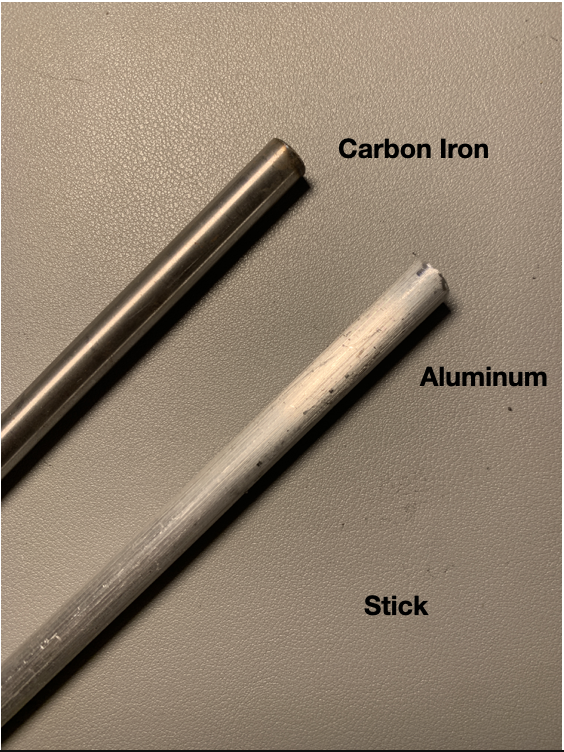
\includegraphics[width=6cm]{stick.png}
\caption{Iron Stick \& Aluminnum Stick}
\label{Stick}
\end{minipage}
\begin{minipage}[t]{0.48\textwidth}
\centering
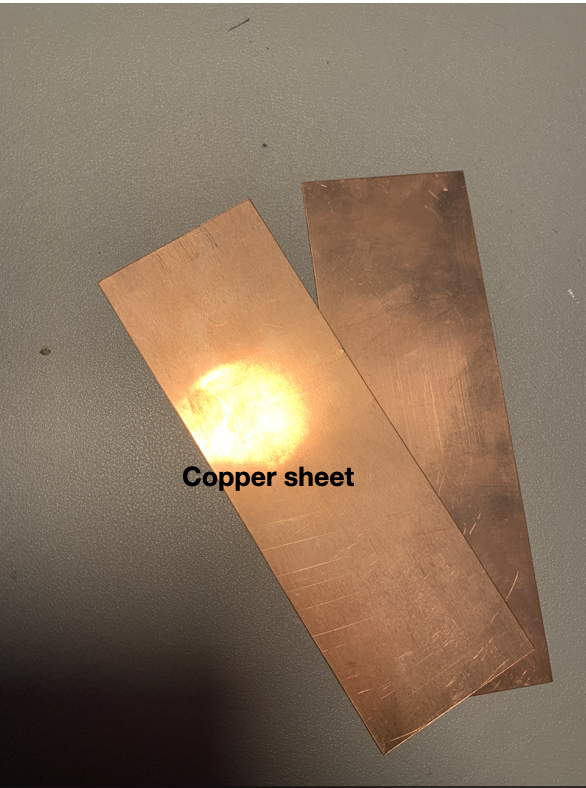
\includegraphics[width=6cm]{sheet.png}
\caption{Copper Sheet}
\label{Sheet}
\end{minipage}
\end{figure}

In experiment,we use 2 kinds of sensor form.One is the waterproof form which is already installed in a waterproof sleeve, which will be used in monitoring the temperature of heat source, water.Another is direct the sensor, which will be installed into the parts and fix and contact to measure the temperature.

\begin{figure}[H]%H为当前位置,!htb为忽略美学标准,htbp为浮动图形
\centering %图片居中
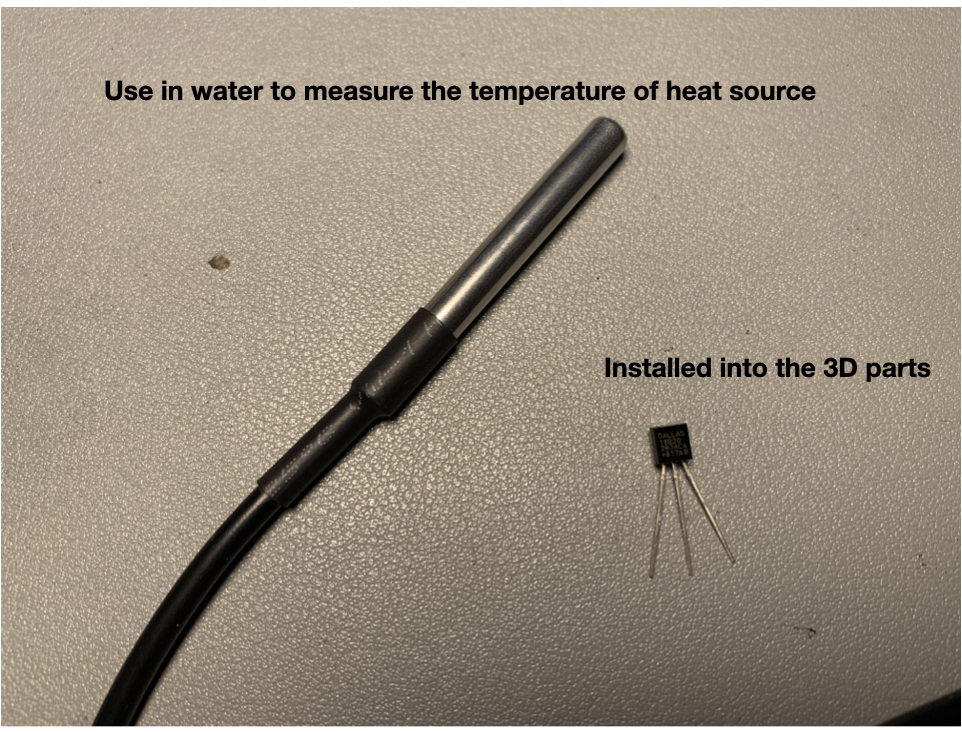
\includegraphics[width=0.5\textwidth]{sensor.png} %插入图片,[]中设置图片大小,{}中是图片文件名
\caption{Sensors} %最终文档中希望显示的图片标题
\end{figure} 

This is the 3D simulation image of the experimental facility \ref{all}. In this image, you can see that the red part is the part I designed that needs 3D printing, which is used to fix and assemble the experimental object and sensor

\begin{figure}[H]%H为当前位置,!htb为忽略美学标准,htbp为浮动图形
\centering %图片居中
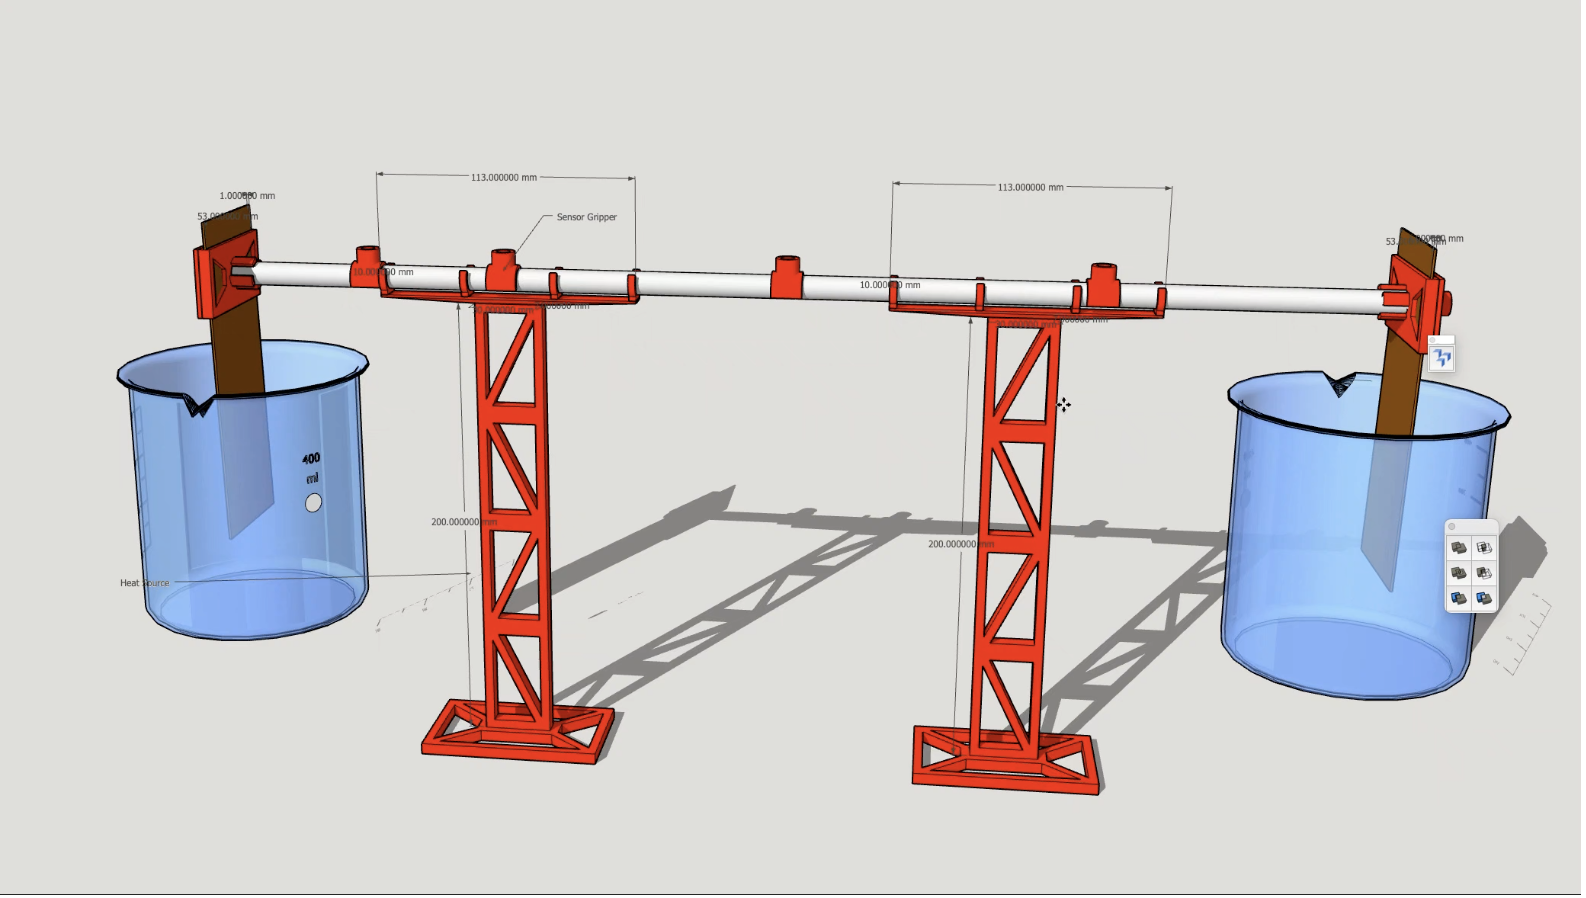
\includegraphics[width=1\textwidth]{all.png} %插入图片,[]中设置图片大小,{}中是图片文件名
\caption{All Instruments(with 3D parts red)} %最终文档中希望显示的图片标题
\label{all}
\end{figure} 




The 3D parts include the support stand \ref{stand} for fixing the metal rod, the sheet stick connector \ref{connector} for connecting the metal rod to the copper sheet, the sheet fixer \ref{fixer} for holding the copper sheet and mounting the sensor at both ends, and the sensor plier \ref{plier} for fixing the sensor to the metal rod, These main parts are made of resin or nylon to prevent melting due to high temperature.


\begin{figure}[H]%H为当前位置,!htb为忽略美学标准,htbp为浮动图形
\centering %图片居中
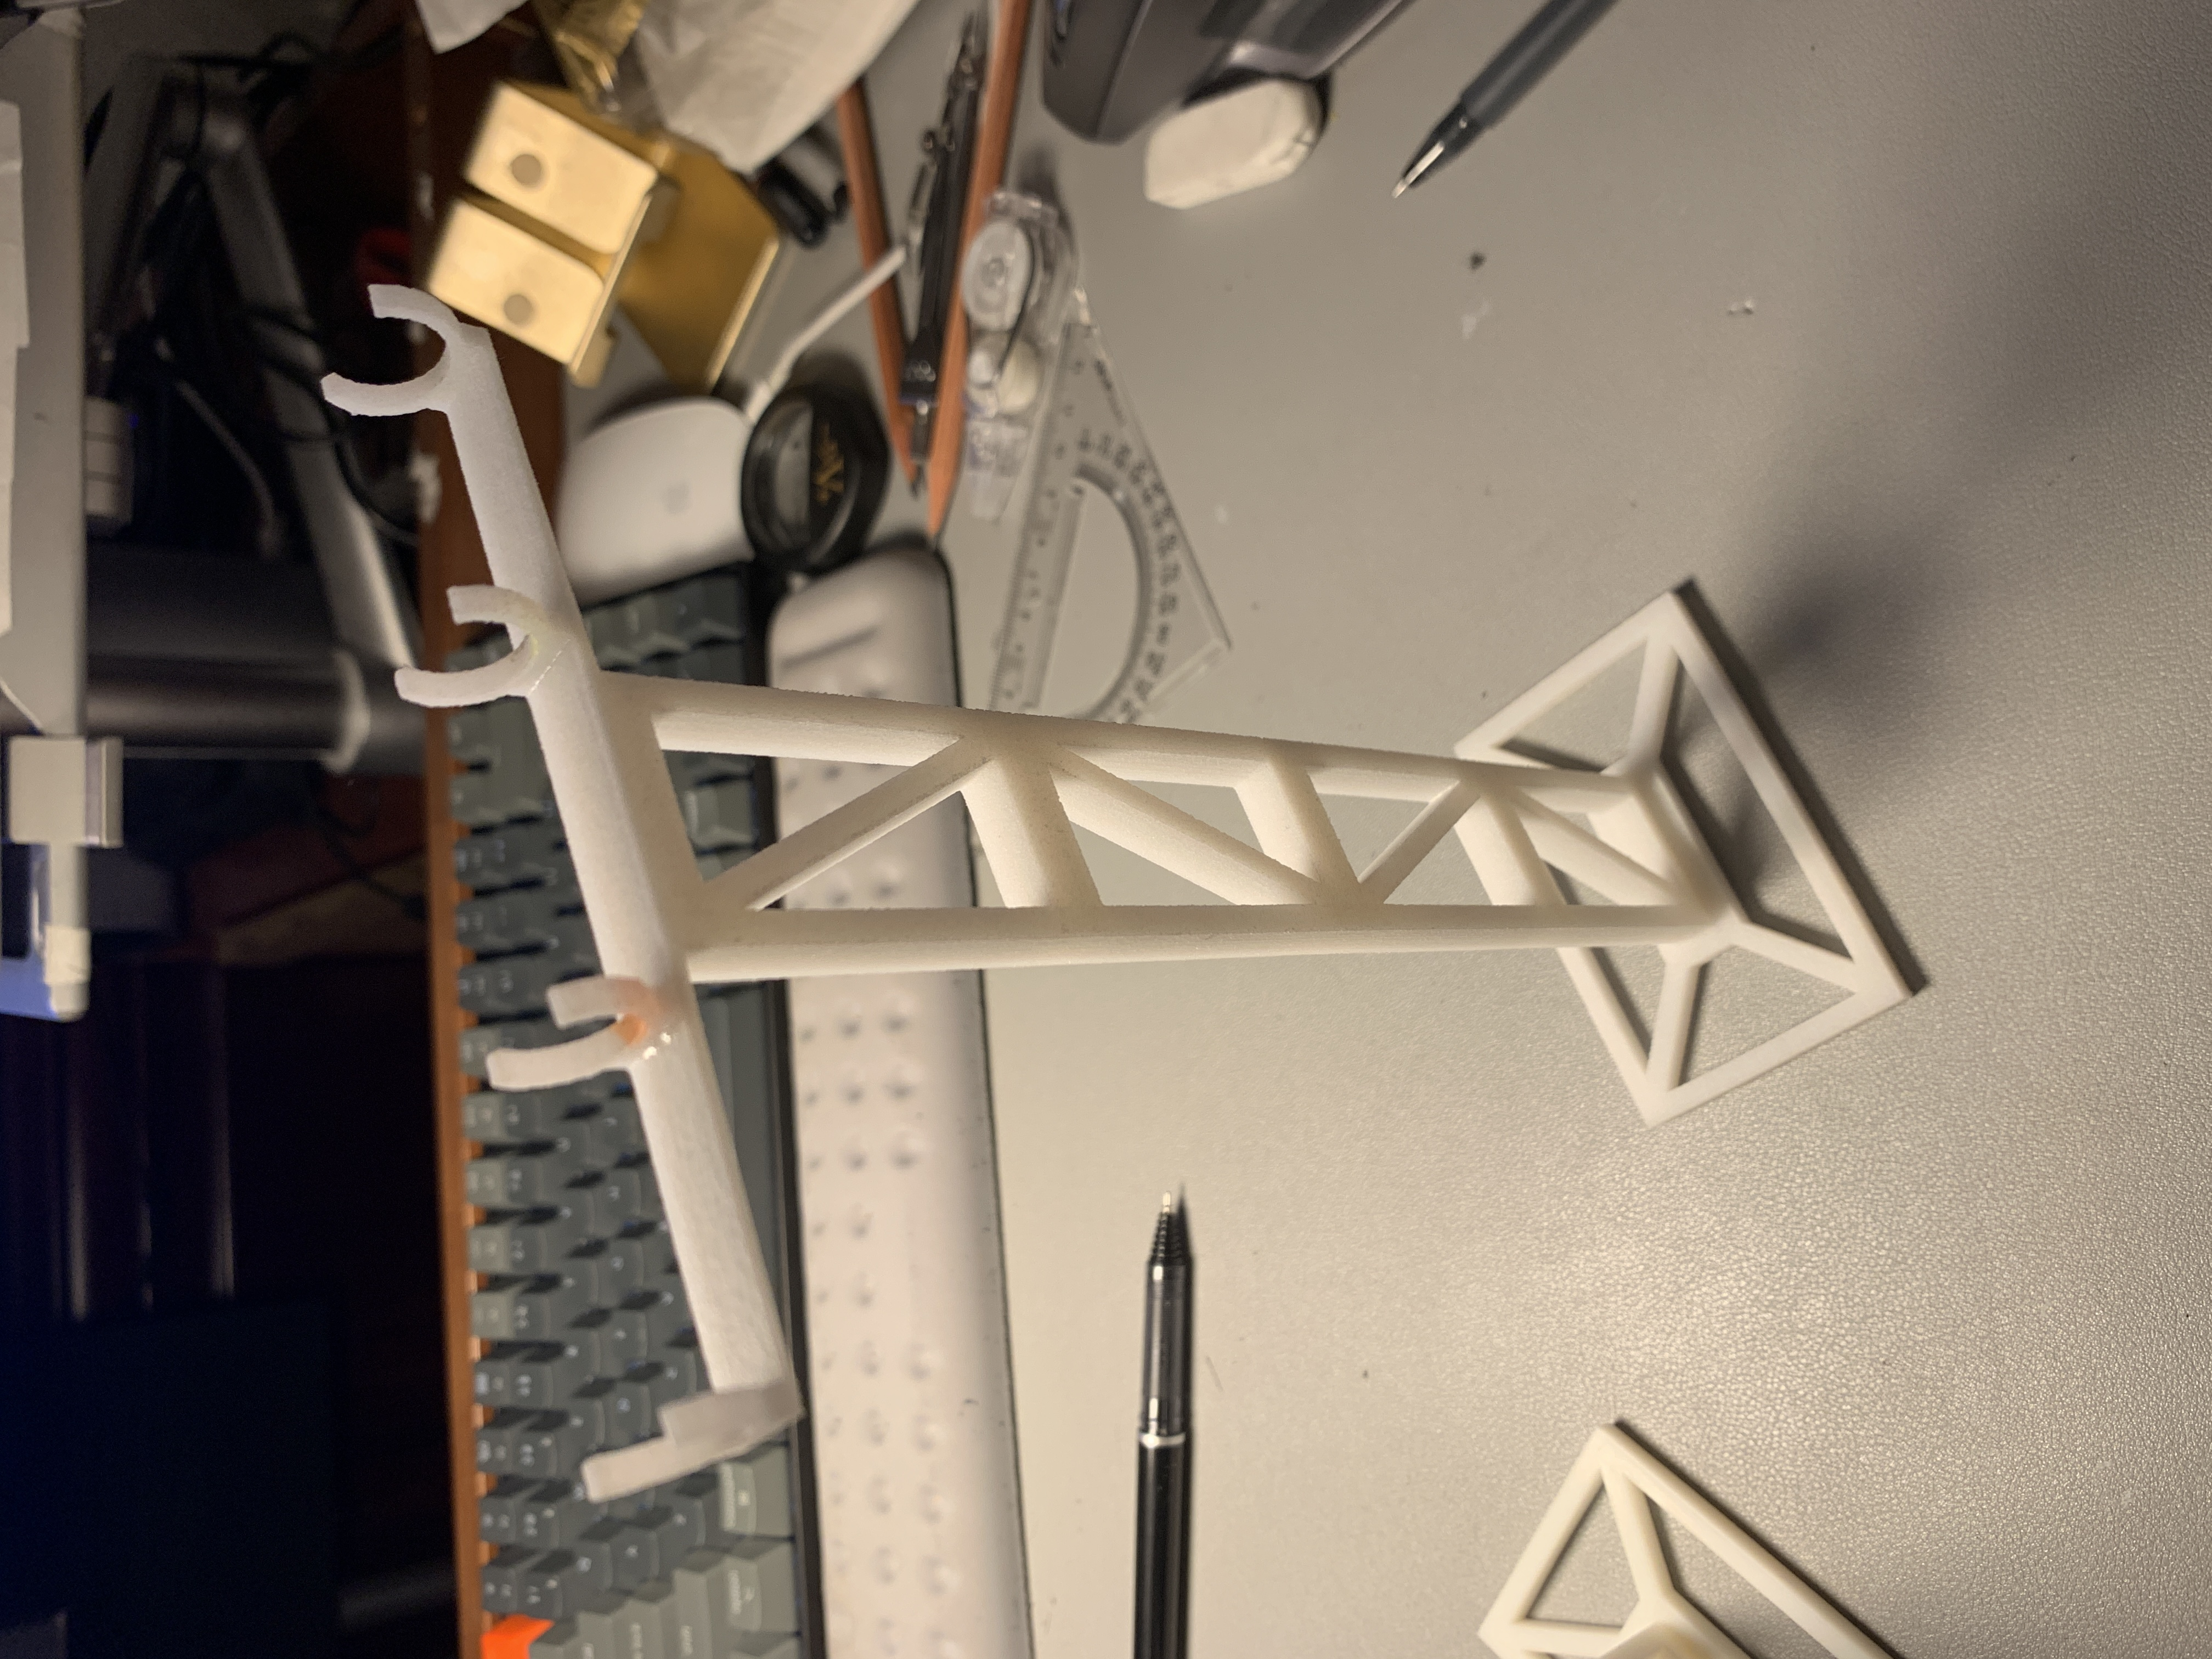
\includegraphics[width=0.5\textwidth,angle=270]{support.JPG} %插入图片,[]中设置图片大小,{}中是图片文件名
\caption{Support Stand} %最终文档中希望显示的图片标题
\label{stand} 
\end{figure}


\begin{figure}[htbp]
\centering
\begin{minipage}[t]{0.3\textwidth}
\centering
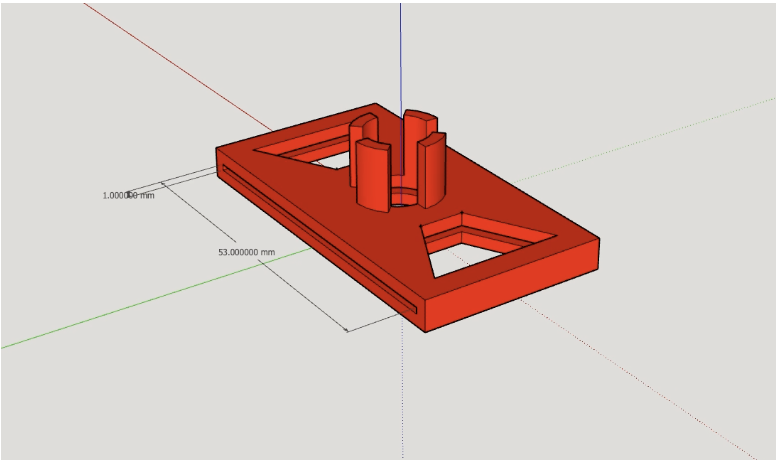
\includegraphics[width=6cm]{connector.png}
\caption{Sheet Stick Connector}
\label{connector}
\end{minipage}
\begin{minipage}[t]{0.3\textwidth}
\centering
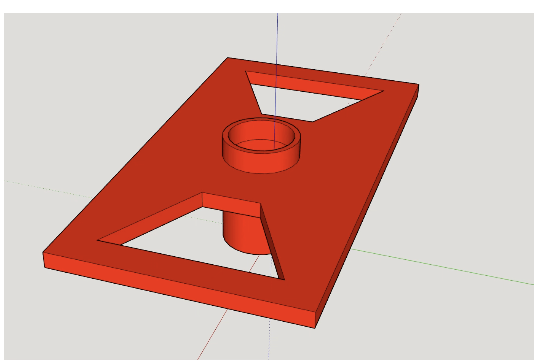
\includegraphics[width=6cm]{fixer.png}
\caption{Sheet Fixer}
\label{fixer}
\end{minipage}
\begin{minipage}[t]{0.3\textwidth}
\centering
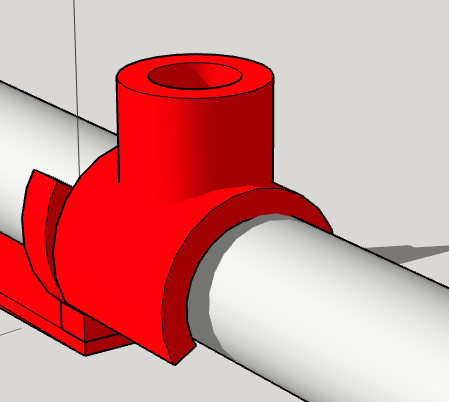
\includegraphics[width=6cm]{plier.png}
\caption{Senor Plier}
\label{plier}
\end{minipage}
\end{figure}



\subsubsection{Program Detailed}

We have written an program to let the sensors and Arduino collect data and send to computer, plot the graph at the same time with the aid of MATLAB, Further details, we shown it by recording a video. refered to the video \href{https://b23.tv/ADx0Op}{https://b23.tv/ADx0Op} 

\subsection{Virtual Experiment Method}



In this experiment, parallel virtual experiments are used as auxiliary and control. In this experiment, we use the finite element physical field simulation software COMSOL \ref{COMSOL} as our main software. He will simulate and analyze the unsteady heat conduction experiment by solving the numerical interpretation of the following formula

\begin{equation}
	\rho C_{\rho} \frac{\partial T}{\partial t}+\rho C_{\rho} \mathbf{u} \cdot \nabla T+\nabla \cdot \mathbf{q}=Q+Q_{\mathrm{ted}}
\end{equation}

\begin{figure}%H为当前位置,!htb为忽略美学标准,htbp为浮动图形
\centering %图片居中
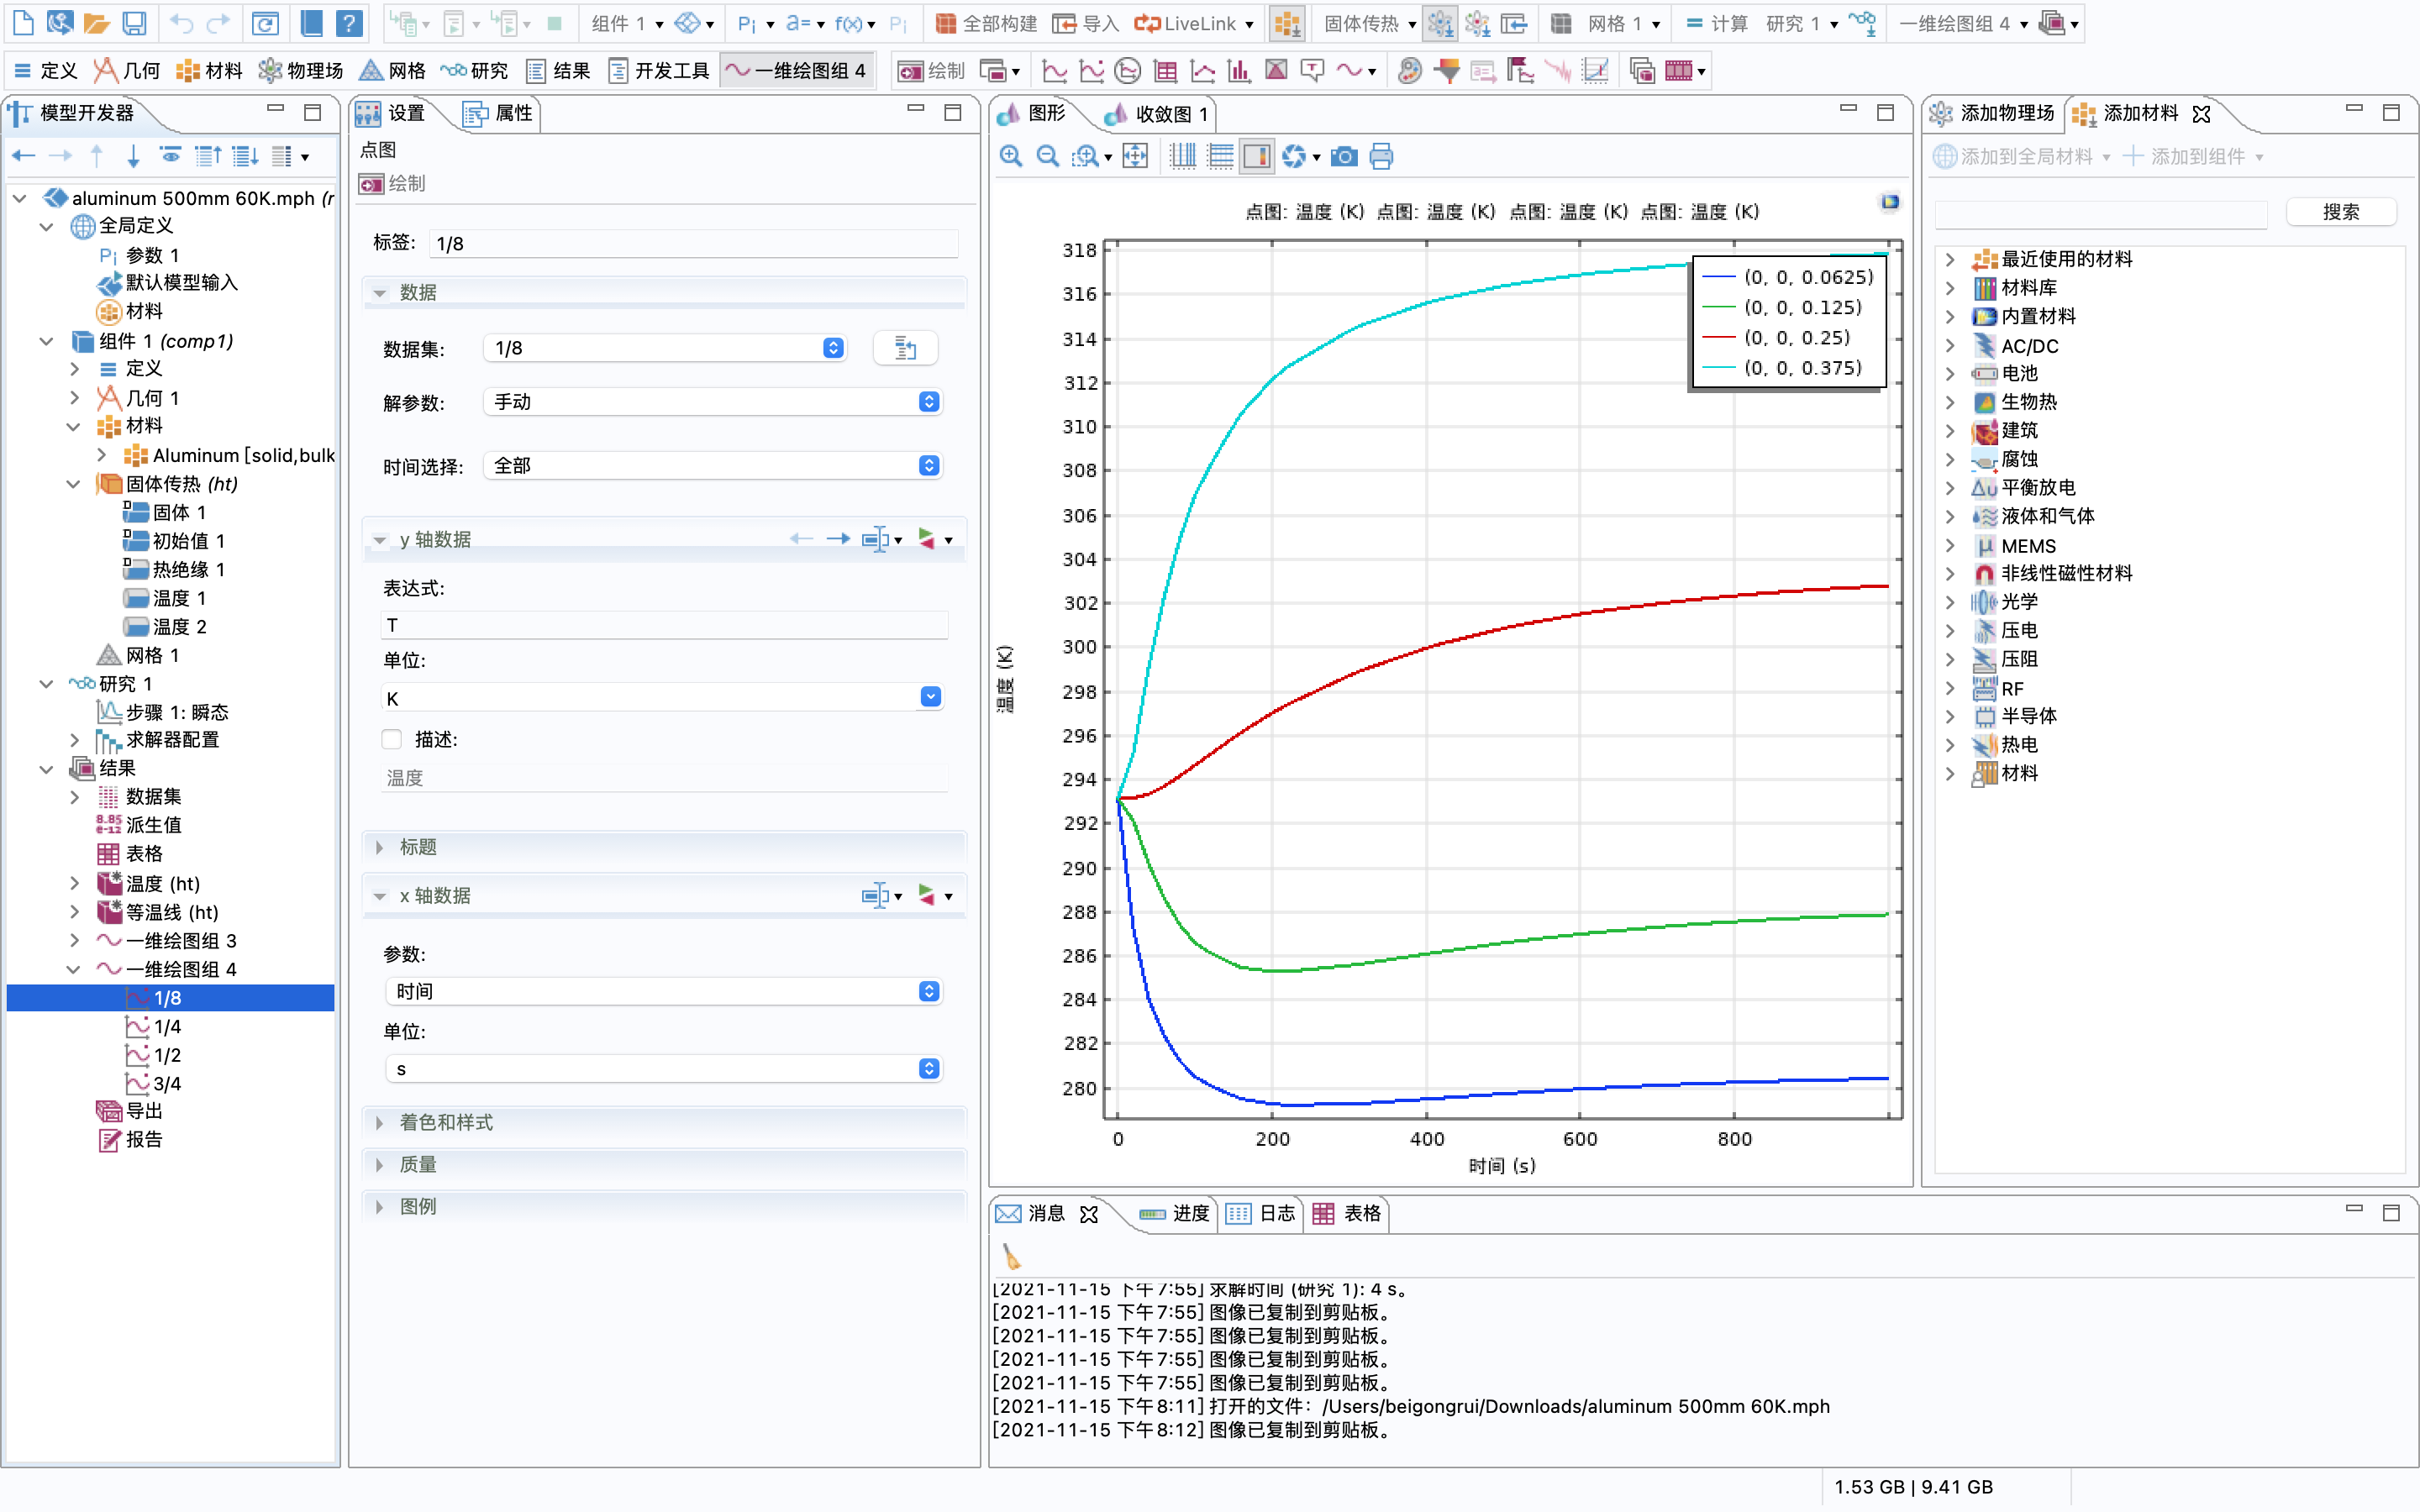
\includegraphics[width=1\textwidth]{COMSOLinterface.png} %插入图片,[]中设置图片大小,{}中是图片文件名
\caption{COMSOL inferface} %最终文档中希望显示的图片标题
\label{COMSOL} 
\end{figure} 

\subsubsection{Virtual experiment operation}
First do the experiment of Aluminium 250mm
\begin{enumerate}
  \item Construct a 5mm radius and 250mm length cylinder, and select "Aluminum [solid,bulk]" as the material.  
  \item Set the initial temperature is 293.15K, set the temperature of the cylinder bottom surface is 273K.  
  \item Set the temperature of the cylinder top surface is 333K.  
  \item Set "time step" of "unsteady state" in the "research" is (0,20,1000), click"calulate".    
  \item Set the length of the sectional line is the whole length of the cylinder, and set four sectional points:1/8,1/4,1/2,3/4 in the "data set".  
  \item Set a "point diagram" in "one-dimensional plot", choose the whole length in the data set. Click "plot".  
  \item Set another four "point diagram" in"one-dimensional plot", choose 1/8,1/4,1/2,3/4 in the "data set", respectively. Click "plot".  
  \item Put all ploting data to shear plate, and derive them to one file.   
  \item Plot "two-dimensional" figures in Excel according to the data in files.  
  \item Change the the temperature of the cylinder top surface to "343K, 353K, 363K, 373K", respectively. And do the follow steps.  
  \item Obeserve the pictures in Comsol and Excel, then analyze them to verify our hypotheses.
\end{enumerate}

Next change the material into Fe:
\begin{enumerate}
  \item Construct a 5mm radius and 250mm length cylinder, and select "Iron[solid,0.00025/s strain rate]" as the material.  
  \item Then repeat the steps in "1)Aluminum 250mm".
\end{enumerate}

Finally Change the length into 500mm


\begin{enumerate}
  \item Construct a 5mm radius and 500mm length cylinder, and select "Aluminum [solid,bulk]" as the material.  
  \item Then repeat the steps in "1)Aluminum 250mm".
\end{enumerate}


\subsection{Detailed steps for verify the hypotheses}
\subsubsection{Hypothesis 1}
Before reaching the steady-state, the speed of temperature change at the point becomes faster with the enhancement of thermal conductivity of the material.   

 
steps: choose a fixed sectional point, keep the temperature difference and the length of the cylinder same, compare the slopes of the "two-dimensional" figures in Excel of different material (aluminum and iron).
\subsubsection{Hypothesis 2}
Before reaching a steady-state, the speed of temperature change at the point becomes faster with the shortening of the metal length.  

  
steps: choose a fixed sectional point, keep the temperature difference and material of the cylinder constant. Change the length of the cylinder (aluminum 250mm and 500mm). Compare the slopes of the "two-dimensional" figures in Excel of different length.
\subsubsection{Hypothesis 3}
Before reaching the steady-state, the speed of temperature change at the point becomes faster with the increase of heat source temperature.  

   
steps: choose a fixed sectional point, keep material and length of the cylinder constant. Change the temperature difference.Compare the slopes of the "two-dimensional" figures in Excel of different temperature difference.

\section{Result \& Discussion}

\subsection{Observations}

\begin{enumerate}
  \item The temperature of the points which are closer to the lower temperature will decrease first and then increase. Seen in \ref{Oberservation1} The two below curve. Which is hard to analyze its data.



\begin{figure}[H] %H为当前位置,!htb为忽略美学标准,htbp为浮动图形
\centering %图片居中
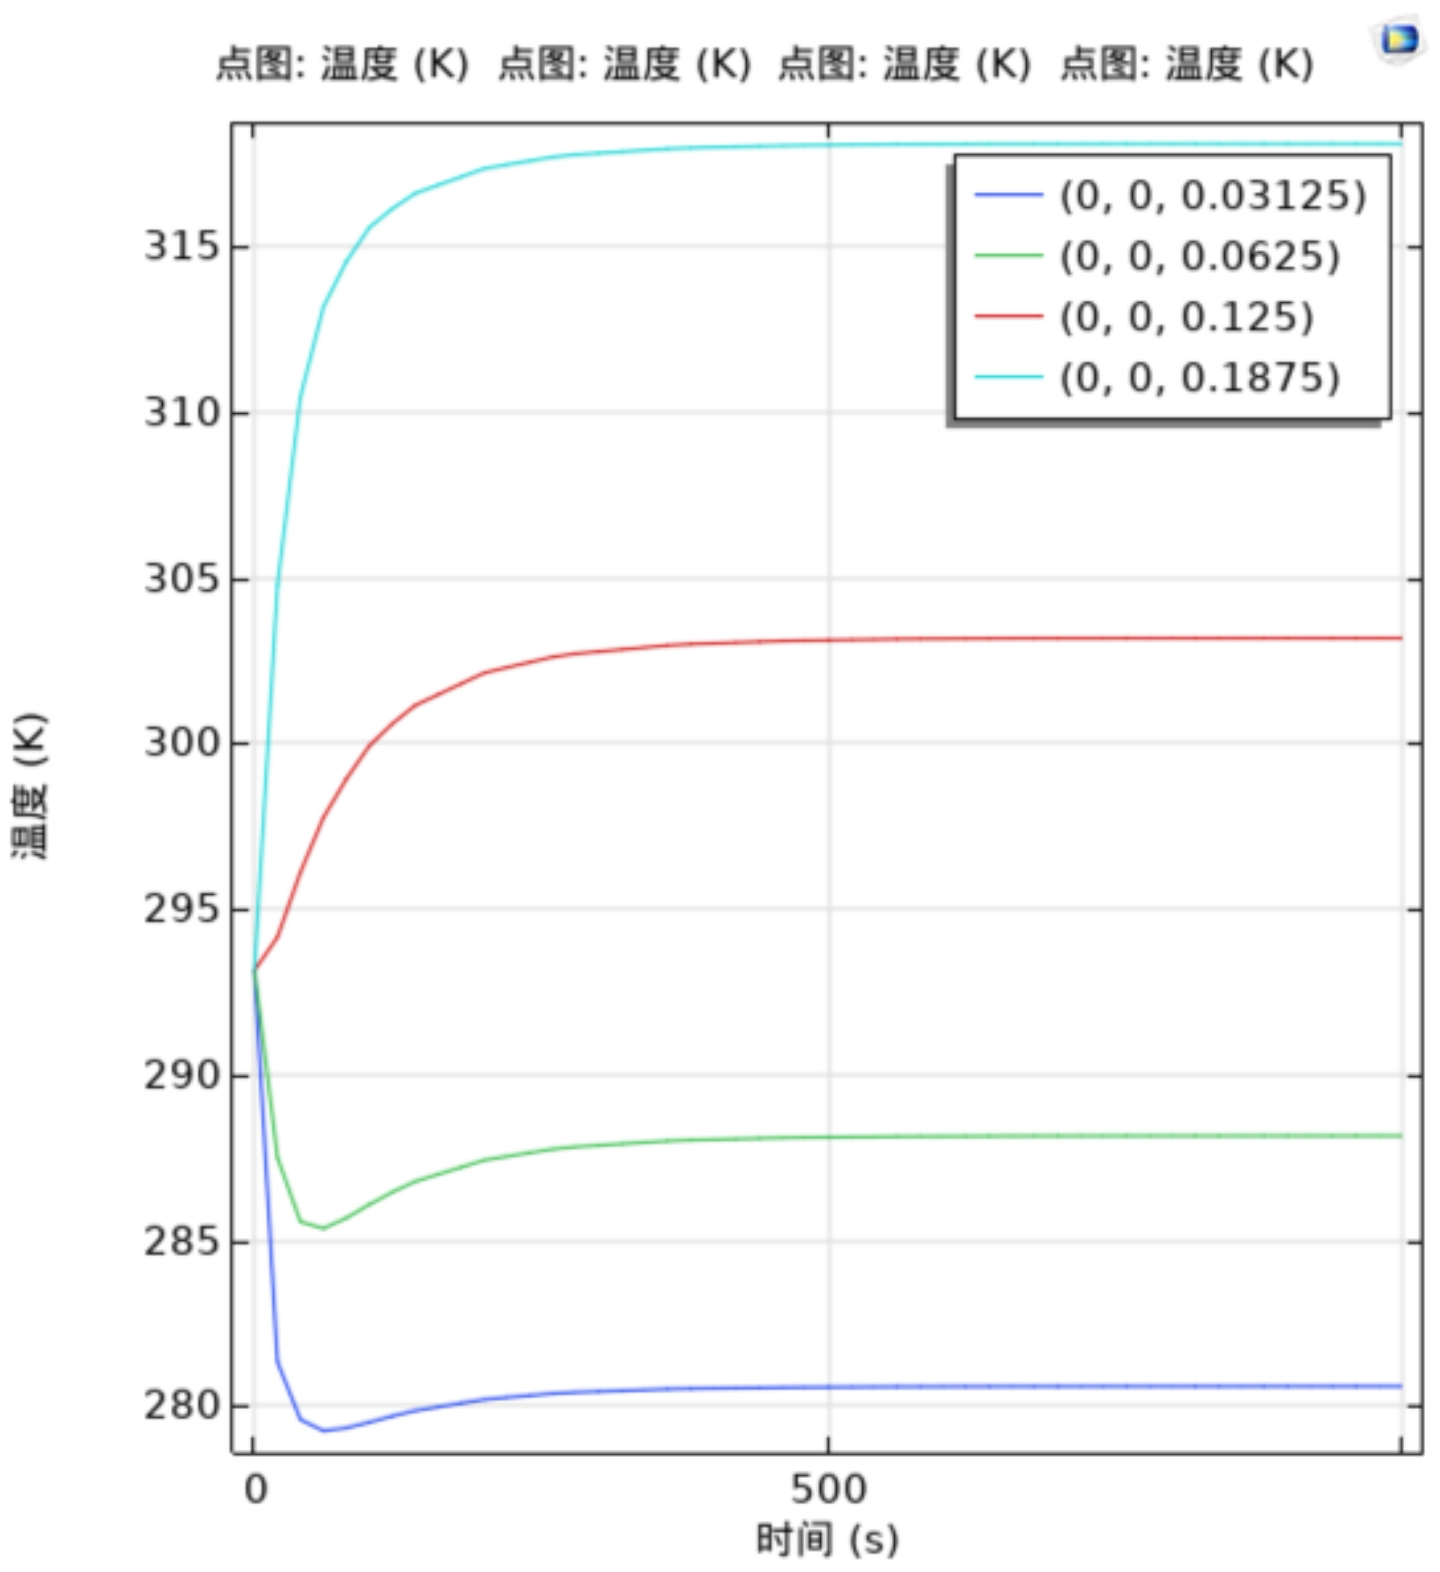
\includegraphics[width=0.5\textwidth]{Observation1.png} %插入图片,[]中设置图片大小,{}中是图片文件名
\caption{Observation 1} %最终文档中希望显示的图片标题 
\label{Oberservation1}
\end{figure} 

\item The temperature increases linearly first and then gradually flattens, similar to the exponential equation.
  \item All temperature of all four points will finally reach the steady state.
  \item The final steady-state temperature corresponding to all points increases as the distance from the origin increases,which is actually linear distributed finally,which is also called as Fourier's Law in thermal equilibrium.
 
 
 \begin{figure}[H] %H为当前位置,!htb为忽略美学标准,htbp为浮动图形
\centering %图片居中
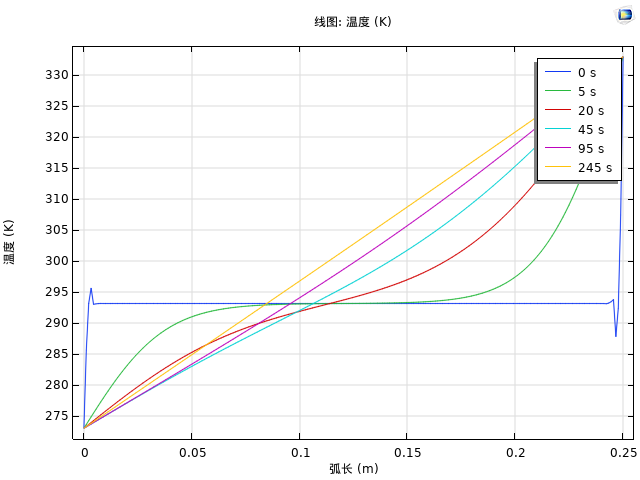
\includegraphics[width=0.5\textwidth]{Observation3.png} %插入图片,[]中设置图片大小,{}中是图片文件名
\caption{Observation 3} %最终文档中希望显示的图片标题 
\end{figure} 

 \item At the initial time, two peaks \ref{3.1} appear in the two sections of the de curve. These two peaks may be due to the deviation of the numerical solution, which we ignore in the experiment.
  \begin{figure}[H] %H为当前位置,!htb为忽略美学标准,htbp为浮动图形
\centering %图片居中
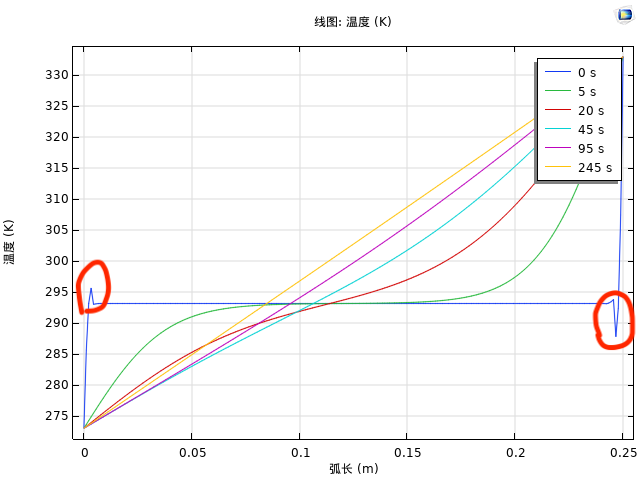
\includegraphics[width=0.5\textwidth]{Observation4.png} %插入图片,[]中设置图片大小,{}中是图片文件名
\caption{Observation 4} %最终文档中希望显示的图片标题 
\end{figure} 
 
 
 
\end{enumerate}

\subsection{Data processing method}
In this experiment, the dependent variable we explore is the speed of temperature change. Therefore, it is worth noting how to measure the speed of temperature change. In this data analysis, we will mainly compare two change speeds. One is the maximum slope of temperature in the whole change process, that is, the maximum temperature change rate; 


The second is the average slope of temperature in the whole change process. When determining this value, we need to first determine when the experiment ends, that is, the temperature will not change sharply. We set this index at 0.01K/s, which means if the temperature doesn't change more than 0.01 degree per second.We will regard the system got equilibrium,the experiment end. By using this point we seperate the data into two part.The first part is the temperature change stage and the second part is stationary part.We calculate the average rate in temperature change stage as our average slope of temperature. 



In the subsequent analysis, we will mainly use these two indicators as our standard to measure the fast full temperature change.






\subsection{Hypothesis 1}
Before discussing the results of hypothesis 1, it is necessary to clarify the concept of thermal conductivity rate.By Wikipedia %TODO 这里引用一下wikipedia
, thermal conductivity rate could be simply defined by \ref{fourier} :
\begin{equation}
	q=-k \cdot \frac{T_{2}-T_{1}}{L} \label{fourier}
\end{equation}
\begin{figure}[H] %H为当前位置,!htb为忽略美学标准,htbp为浮动图形
\centering %图片居中
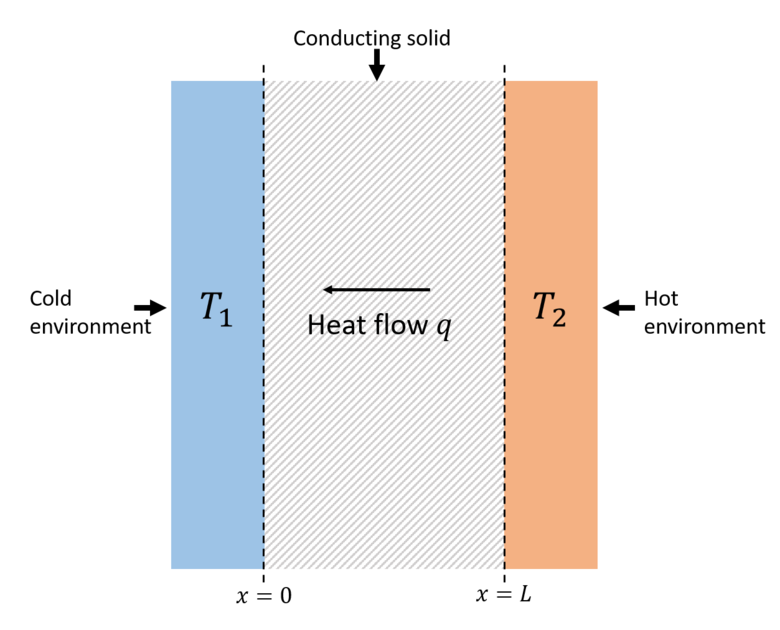
\includegraphics[width=.5\textwidth]{ThermalTransfer.png} %插入图片,[]中设置图片大小,{}中是图片文件名
\caption{Thermal transfer Diagram} %最终文档中希望显示的图片标题
\end{figure}\label{Heattranfer}


The thermal conductivity of a material is a measure of its ability to conduct heat. Generally speaking, metals have better thermal conductivity, which means that metals can transport more heat at the same time. By consulting the metal thermal conductivity data in COMSOL, we can find the following data  :


% Please add the following required packages to your document preamble:
% 
% If you use beamer only pass "xcolor=table" option, i.e. \documentclass[xcolor=table]{beamer}
\begin{table}[H]
\centering
\begin{tabular}{|c|c|}
\hline

\textbf{Metal type} & Thermal Conductivity Rate(Wm\textasciicircum{}-1K\textasciicircum{}-1) \\ \hline
\textbf{Aluminum}   & 237                                                                    \\ \hline
\textbf{Steel}      & \cellcolor[HTML]{F8F9FA}{\color[HTML]{202122} 80}                      \\ \hline


\end{tabular}
\end{table}


Here, we first take the temperature change data of $250mm$ aluminum and iron at $1 / 2$ of the whole length at the room temperature of $20 ^\circ C$, $0 ^\circ C$ at one end and $100 ^\circ C$ at the other end,and campare it with the Fe in same situation and same sampling point.


We have not fully completed the data analysis of this hypothesis, and further reports will be presented in the future.

\subsection{Hypothesis 2}
In this hypothesis, due to the change of length, we can have two understandings of the same position. First, the position in proportion, such as the midpoint; The second understanding is the same point in distance, such as 125mm from the heat source. Therefore, we analyze these two understandings separately here.


Firstly, we assume that it is the same point in proportion, so we extract the temperature change of aluminum under the conditions of 500mm and 250mm:
\begin{figure}[H] %H为当前位置,!htb为忽略美学标准,htbp为浮动图形
\centering %图片居中
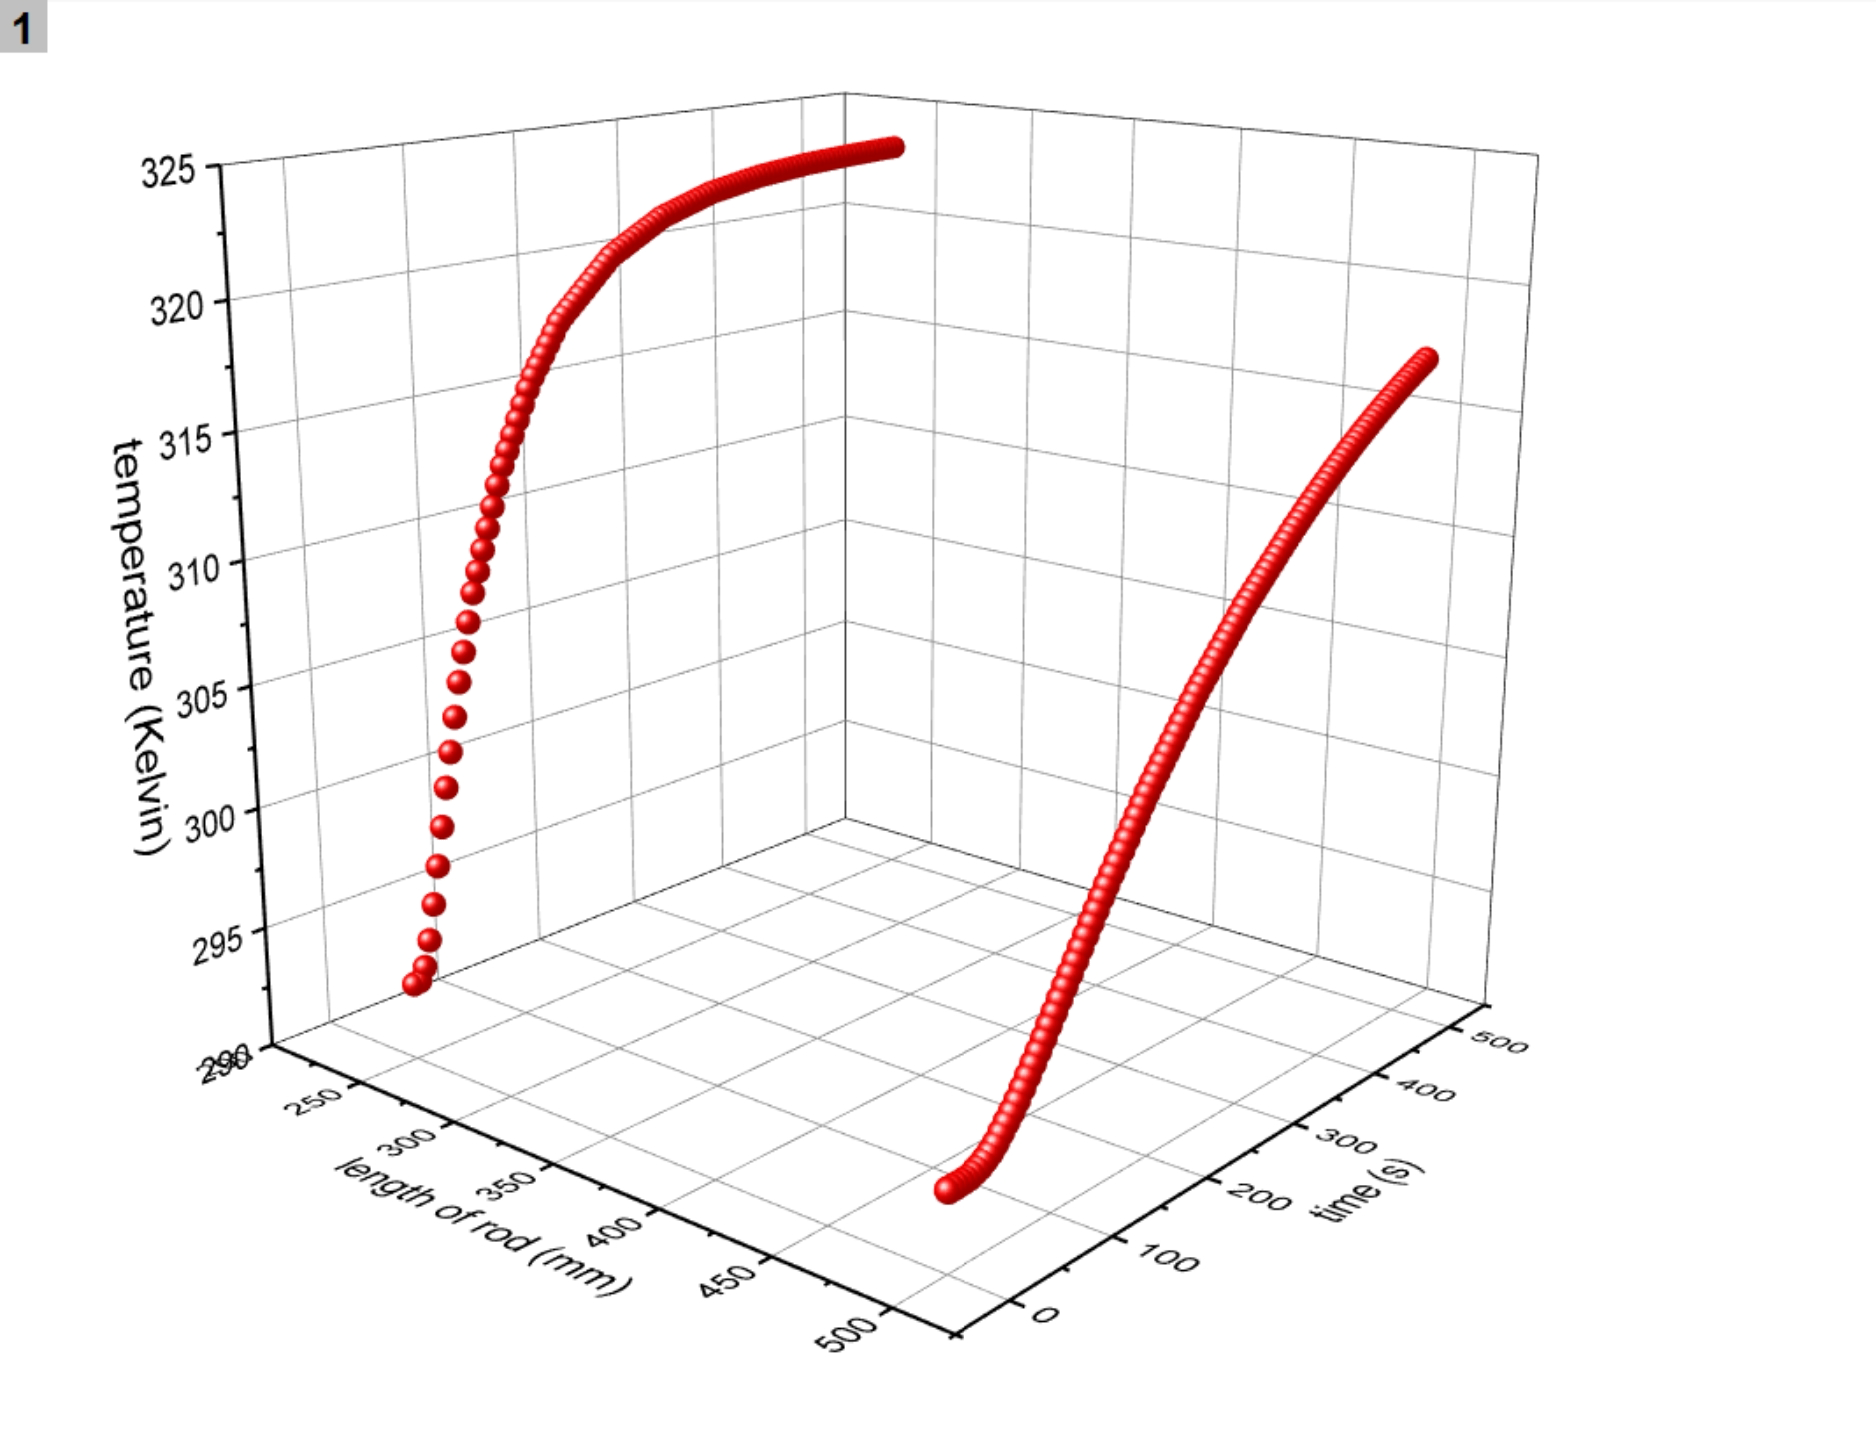
\includegraphics[width=0.5\textwidth]{Hypothesis_2_1.png} %插入图片,[]中设置图片大小,{}中是图片文件名
\caption{Maximum Point} %最终文档中希望显示的图片标题 
\end{figure} 


The left hand side’s curve represents the temperature of the center point of 250mm Aluminum rod, and the right hand side’s curve represents 500mm’s. It’s obvious to see that the 250mm’s Aluminum rod possesses a shorter time to reach the thermal equilibrium.

Because the shorter the cylinder is, the faster the speed of temperature change is. Then the hypothesis 2 is correct.




We have not fully completed the data analysis of this hypothesis, and further reports will be presented in the future

\subsection{Hypothesis 3}
First, take a visual look \ref{3.1} at the three-dimensional image of temperature change drawn on Aluminum, 250mm, midpoint and high-temperature end between 60 ℃ and 100 ℃ in 0 to 500s.


\begin{figure}[H] %H为当前位置,!htb为忽略美学标准,htbp为浮动图形
\centering %图片居中
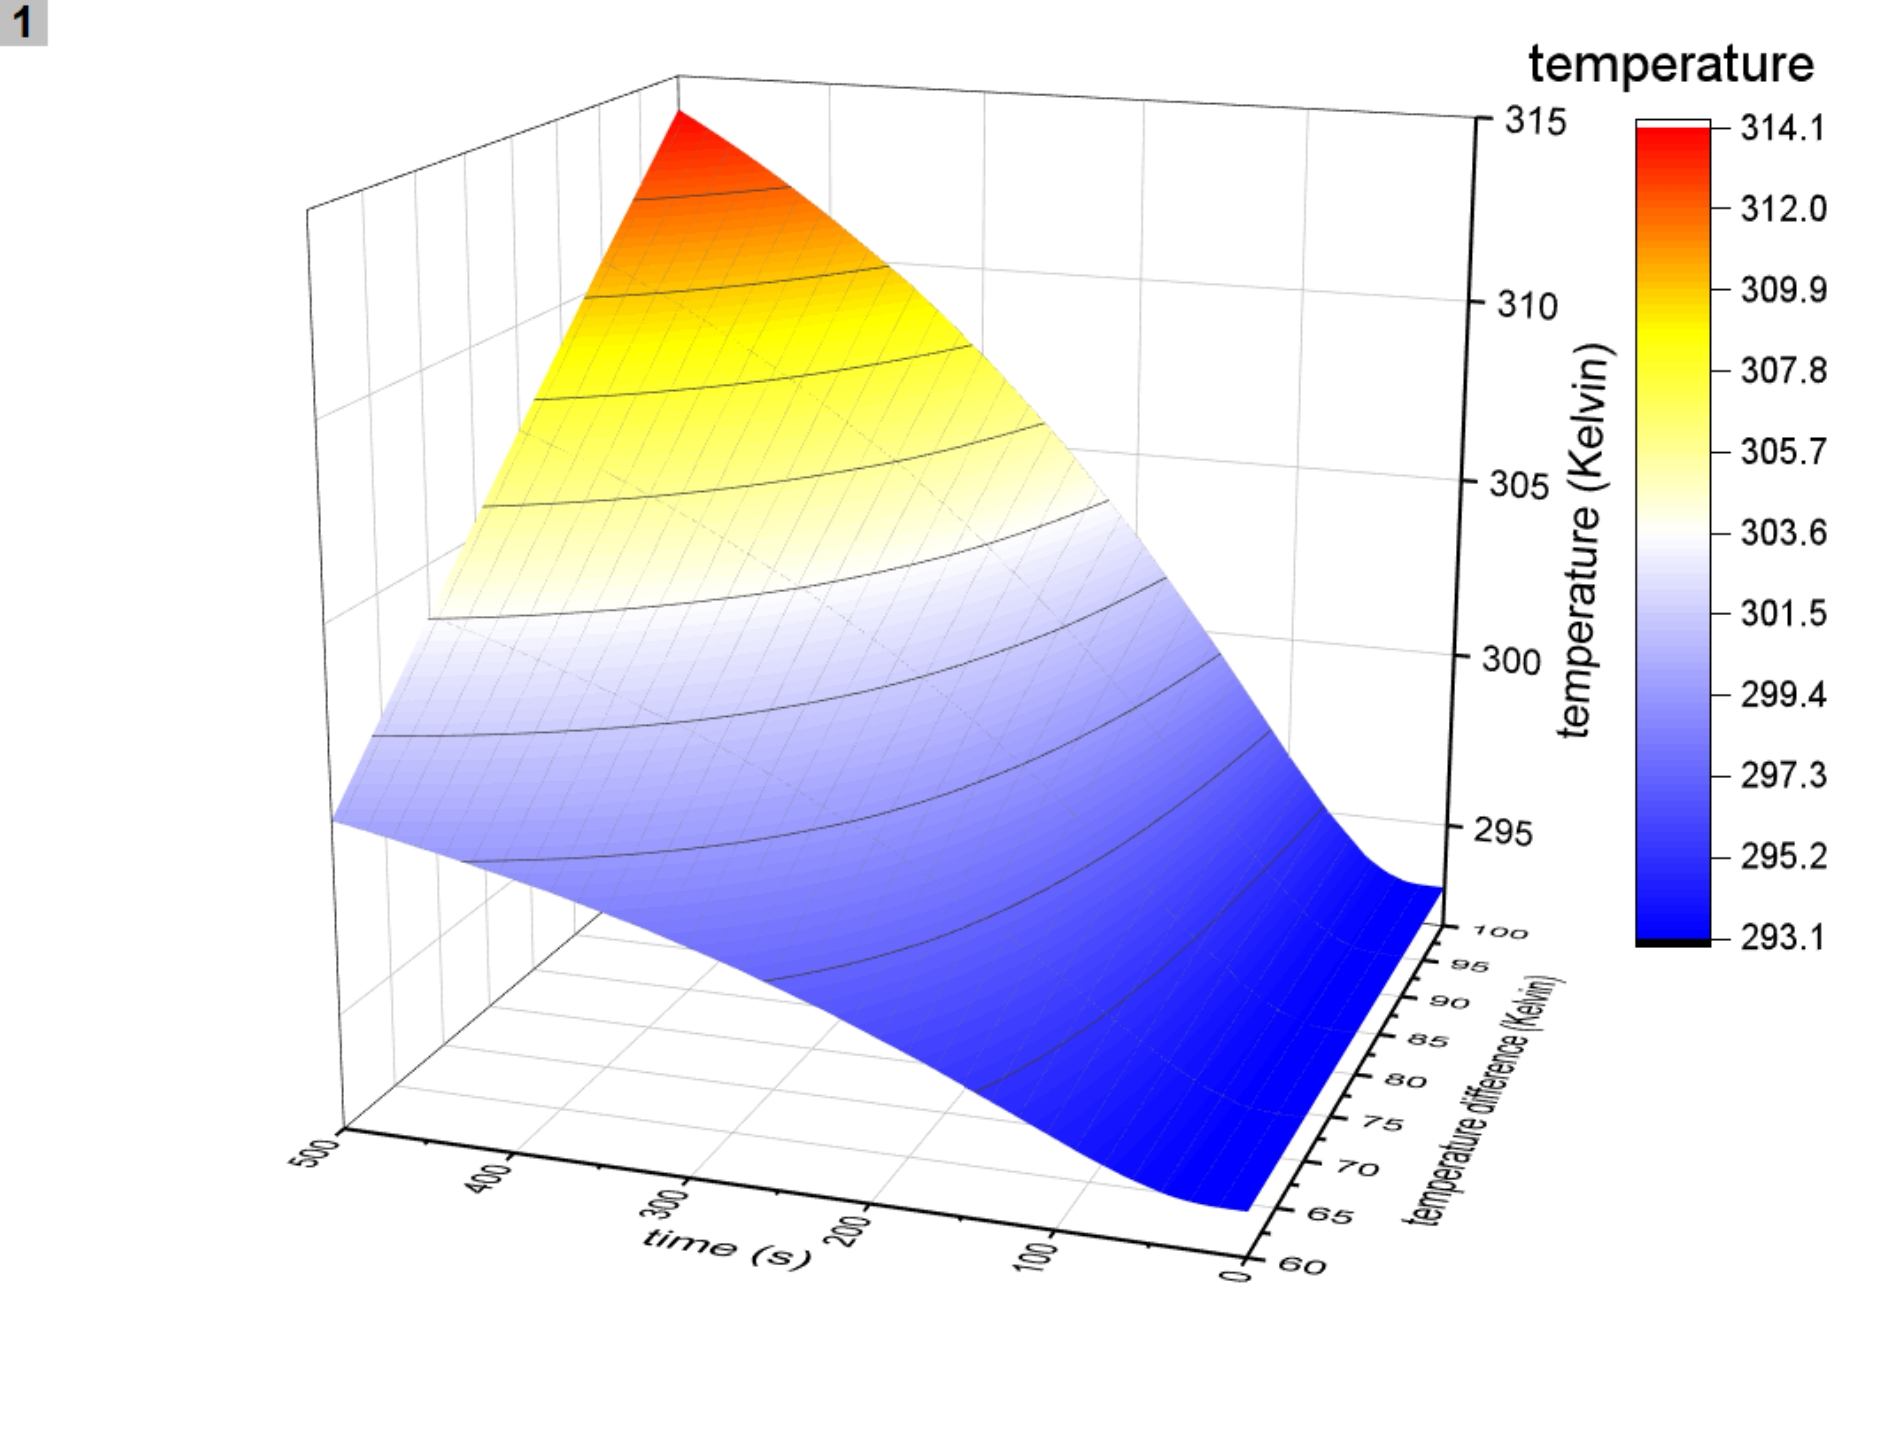
\includegraphics[width=0.5\textwidth]{Hypothesis_3_1.png} %插入图片,[]中设置图片大小,{}中是图片文件名
\caption{Hypothesis 3} %最终文档中希望显示的图片标题 
\label{3.1}
\end{figure} 

There are two axis, one stands for time and the other represents $\Delta T$. It’s obvious to see that, when other variables controlled, larger the $\Delta T$, the slope of the graph during the process of reaching thermal equilibrium is larger.

Because the $\Delta T$ is larger, the speed of temperature change is larger. Then the hypothesis 3 is correct.




Here we look into the detail of the data. Because the temperatures at both ends are not fixed, the steady-state temperatures at these points are different, and it is not meaningful to compare the average change rate. Therefore, here we analyze the relationship between the maximum rate and through the operation of MATLAB. We can get the time, temperature, value and corresponding position of the maximum slope in the figure, as shown in the following figure \ref{Max Point}:



\begin{figure}[H] %H为当前位置,!htb为忽略美学标准,htbp为浮动图形
\centering %图片居中
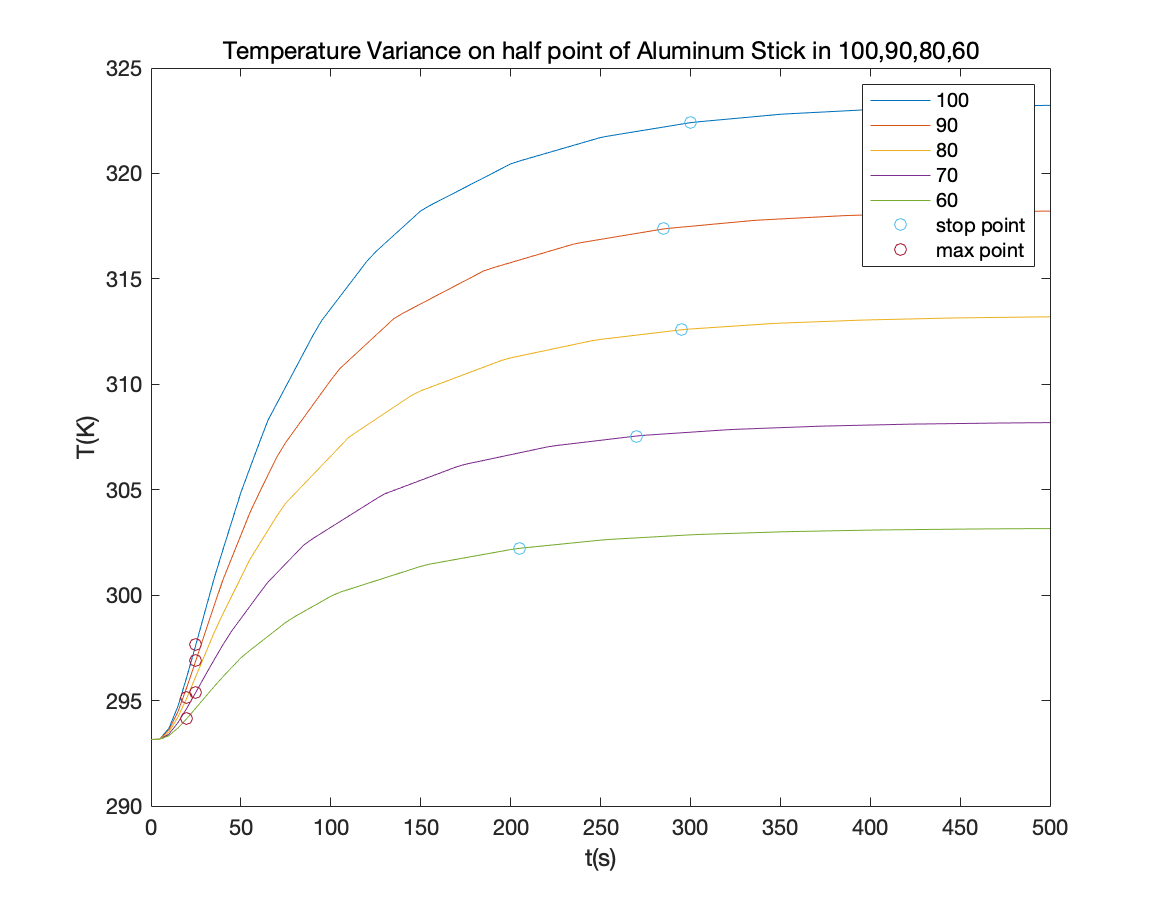
\includegraphics[width=0.5\textwidth]{Hypothesis3_2.png} %插入图片,[]中设置图片大小,{}中是图片文件名
\caption{Maximum Point} %最终文档中希望显示的图片标题 
\label{Max Point}
\end{figure} 


And the chart below:
% Please add the following required packages to your document preamble:
% \usepackage[table,xcdraw]{xcolor}
% If you use beamer only pass "xcolor=table" option, i.e. \documentclass[xcolor=table]{beamer}
\begin{table}[h]
\centering
\begin{tabular}{|c|c|l|l|l|l|}
\hline
\rowcolor[HTML]{C0C0C0} 
\cellcolor[HTML]{9B9B9B}{\color[HTML]{000000} \textbf{Temperature}} & {\color[HTML]{000000} \textbf{100K}}                  & {\color[HTML]{000000} \textbf{90K}} & {\color[HTML]{000000} \textbf{80K}} & {\color[HTML]{000000} \textbf{70K}} & {\color[HTML]{000000} \textbf{60K}} \\ \hline
\cellcolor[HTML]{9B9B9B}\textbf{Max Slope Time}                     & 25                                                    & 25                                  & 20                                  & 25                                  & 20                                  \\ \hline
\cellcolor[HTML]{9B9B9B}\textbf{Max Slope Temperature}              & \cellcolor[HTML]{F8F9FA}{\color[HTML]{202122} 297.66} & 296.90                              & 295.13                              & 295.40                              & 294.15                              \\ \hline
\cellcolor[HTML]{9B9B9B}\textbf{Max Slope}                          & \multicolumn{1}{l|}{0.31}                             & 0.26                                & 0.20                                & 0.15                                & 0.10                                \\ \hline
\end{tabular}
\end{table}


It is easy to find that the time to reach the maximum change rate is 20s to 25s, which is not at the beginning of the experiment. This may be because the temperature at the midpoint does not start to rise at the beginning, and it is necessary to wait for the increase of the temperature difference.



By plotting, we can find the relationship between the maximum slope and the heat source temperature. And apply Curve Fitting Tools,we derive that the linear relation between the temperature and Maximum Slope:


\begin{figure}[H] %H为当前位置,!htb为忽略美学标准,htbp为浮动图形
\centering %图片居中
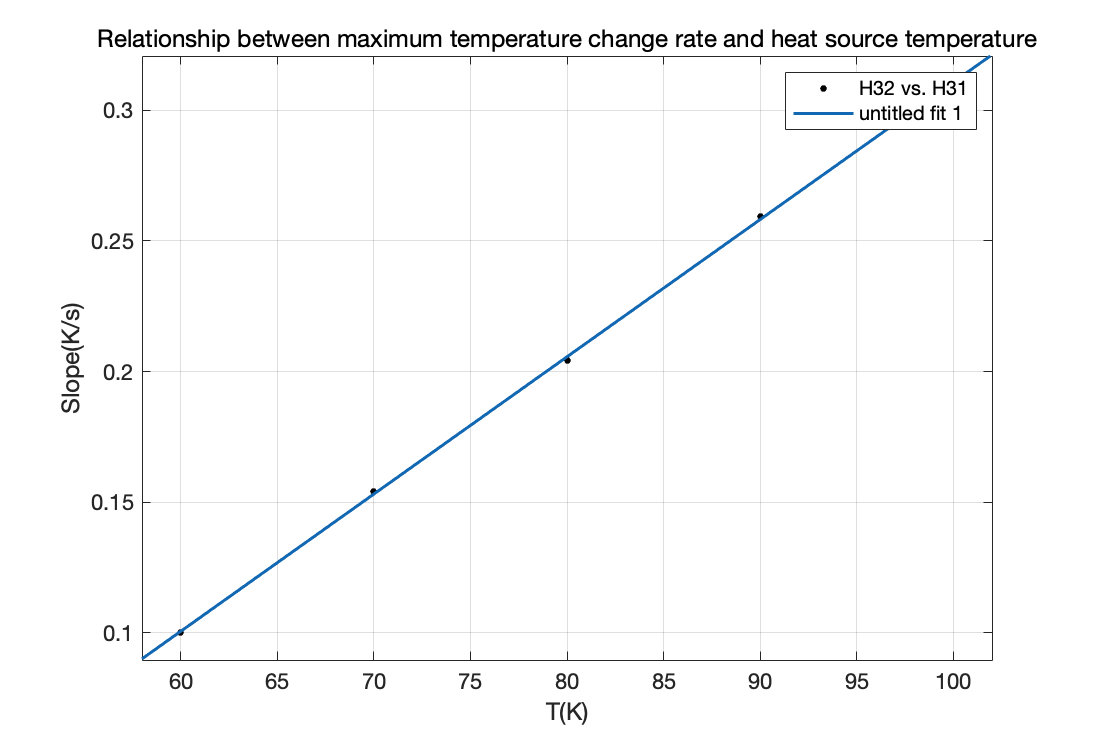
\includegraphics[width=0.5\textwidth]{H3CFT.png} %插入图片,[]中设置图片大小,{}中是图片文件名
\caption{Relationship between maximum temperature change rate and heat source temperature} %最终文档中希望显示的图片标题 
\end{figure} 

 
\begin{lstlisting}
Result of CFTtool
 Linear model Poly1:
 f(x) =pl*x+p2
 where x is normalized by
 Coefficients (with 95 confididence)
 p1= 0.08311
 p2= 0.2056
 Goodness of fit:
 SSE: 4.854e-06
 R-square: 0.9998
 Adjusted R-square: 0.9998
 RMSE: 0.001272
\end{lstlisting}
Therefore, we can find that the two show a very clear linear relationship.













\section{Conclusion \& Recommendation}

\subsection{Conclusion}
Based on our 3 simulation experiments, we conclude 3 result:
\begin{enumerate}
  \item The ratio of temperature change with time will be different with the change of material.Better the thermal conductivity is, faster will the temperature change.
  \item The ratio of temperature change with time will increase with the temperature difference between two sides of the rod increases.
  \item The ratio of temperature change with time will decrease with the length of the metal rod's certain point to the heat source increases.
\end{enumerate}




\subsection{Recommendation}
\begin{enumerate}
  \item The time interval is 5 seconds per point, but for precise data, 5 second is too long, the time interval will be shorten to 1 second.
  \item The range of time is also an issue. 500 seconds can let some of our experiment sets reaches a thermal equilibrium state, but some don’t. For a picture of whole view, we should increase the range of our recording time to 1000 seconds.
  \item More sampling point could be added,to get more precise data
\end{enumerate}




\section{Overall Budget}


We have purchased most of the required materials and tools, and left a sufficient budget to meet the impact of uncertain factors, such as the damage of 3D printing parts and sensors. If necessary, we can purchase more materials from the remaining budget for testing, so as to make the experiment more sufficient.


Below is the budget list before 15th November,2021.The total spending is about RM 244.99. The Snapshot of the Invoice has been uploaded in \href{https://xmueducn-my.sharepoint.com/:f:/g/personal/phy2009481_xmu_edu_my/EvIBnq7mNU1EnrVq51AzZlMBAzm7wgJzyvNK9EDlRcBWUg?e=X8belq}{OneDrive} 


\begin{figure}[H] %H为当前位置,!htb为忽略美学标准,htbp为浮动图形
\centering %图片居中
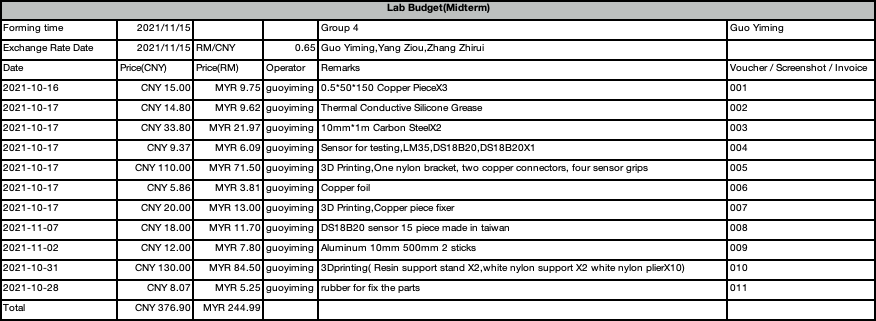
\includegraphics[width=1\textwidth]{MidtermBudget.png} %插入图片,[]中设置图片大小,{}中是图片文件名
\caption{Midterm Budget} %最终文档中希望显示的图片标题 
\end{figure} 








\appendix
      \section{MATLAB Program for Collecting Data(Test Version)}
      \subsection{Function to interpret the signal from DS18B20}
      \begin{lstlisting}
      	function [celsius] = gettemperature(sensor,addr)
reset(sensor);
write(sensor, addr, hex2dec('44'), true);

reset(sensor);
write(sensor, addr, hex2dec('BE')); % read command - 'BE'
data = read(sensor, addr, 9);
crc = data(9);
if ~checkCRC(sensor, data(1:8), crc, 'crc8')
    error('Invalid data read.');
end
raw = bitshift(data(2),8)+data(1);
cfg = bitshift(bitand(data(5), hex2dec('60')), -5);
switch cfg
    case bin2dec('00')  % 9-bit resolution, 93.75 ms conversion time
        raw = bitand(raw, hex2dec('fff8'));
    case bin2dec('01')  % 10-bit resolution, 187.5 ms conversion time
        raw = bitand(raw, hex2dec('fffC'));
    case bin2dec('10')  % 11-bit resolution, 375 ms conversion time
        raw = bitand(raw, hex2dec('fffE'));
    case bin2dec('11')  % 12-bit resolution, 750 ms conversion time
    otherwise
        error('Invalid resolution configuration');
end
% Convert temperature reading from unsigned 16-bit value to signed 16-bit.
raw = typecast(uint16(raw), 'int16');
celsius = double(raw) / 16.0;
fahrenheit = celsius * 1.8 + 32.0;
end

      \end{lstlisting} 
      \subsection{Data Collecting from two sensor in parallel one pin(10)}
\begin{lstlisting}
      	clc
clear
a = arduino('/dev/cu.usbmodem14301','Uno','libraries','PaulStoffregen/OneWire');
sensor = addon(a, 'PaulStoffregen/OneWire', 'D10');
addr = sensor.AvailableAddresses{1};
addr2 = sensor.AvailableAddresses{2};

celsiusdatabase=[];
h1 = animatedline('Color','r');
h2 = animatedline('Color','b');

legend('1st sensor','2nd sensor')
ylim([20 200]);

for hsecond=1:300
pause(0.5)
celsius1=gettemperature(sensor,addr);
celsius2=gettemperature(sensor,addr2)-5;

addpoints(h1,hsecond,celsius1);
addpoints(h2,hsecond,celsius2);

sprintf('Temperature 1 = %.4f Celsius', celsius1)
sprintf('Temperature 2 = %.4f Celsius', celsius2)

xlim([1 max(100,hsecond)]);

drawnow
celsiusdatabase=[celsiusdatabase;[hsecond,celsius1,celsius2]];
end
\end{lstlisting}

      
\section{MATLAB Data Proceding Program(Completed)}
\subsection{get temperature difference}
\begin{lstlisting}
function [Hdiff] = getdiff(Hdata)
% Written By Guo 2021/11/16 
Hdata1=Hdata;
Hdata2=Hdata;

Hdata1(end,:)=[];
Hdata2(1,:)=[]; %shift the data for 1 position
Hdiff=Hdata2-Hdata1; %get the difference
Hdiff(:,1)=[];   
Hdiff=[Hdata1(:,1),Hdiff]; %delete and add the time coordinate.
end
\end{lstlisting}


\subsection{get average slope}
\begin{lstlisting}
function [stoppoint] = getavrate(Hdata,stopslope,startposition)
Hdata1=Hdata;
Hdiff=getdiff(Hdata1);
sizenumber=size(Hdiff);
stoppoint=[];
for i=2:sizenumber(2)
    j=startposition;
    while Hdiff(j,i)>stopslope
        j=j+1;
    end
    avslope=(Hdata(j,i)-Hdata(1,i))/(Hdata(j,1)-Hdata(1,1));
    stoppoint=[stoppoint,[Hdiff(j,1);Hdata1(j,i);avslope]];
end	
\end{lstlisting}


\subsection{get the maximum slope}
\begin{lstlisting}
function [hmax] = getmaxrate(Hdata)
Hdiff=getdiff(Hdata);
sizenumber=size(Hdiff);
Hnumber=sizenumber(2);
hmax=[];
for i=2:Hnumber
    [maxnumber,maxposition]=max(Hdiff(:,i));
    maxslope=maxnumber/(Hdata(2,1)-Hdata(1,1));
    hmax=[hmax,[Hdiff(maxposition,1);Hdata(maxposition,i);maxslope]];
end	
\end{lstlisting}

\section{Hypotheis 3 Data Analysis}
\begin{lstlisting}
hold off
clear 
load Vdata


H3data=[Al250100(:,1),Al250100(:,4),Al25090(:,4),Al25080(:,4),Al25070(:,4),Al25060(:,4)];


H3data1=H3data;
H3data2=H3data;
H3data1(1,:)=[];
H3data2(end,:)=[];
H3diff=[H3data2(:,1),(H3data1-H3data2)/5];
H3diff(:,2)=[];
H3stop=[];
for i=1:5
    test=8;
    while H3diff(test,i+1)>0.01
        test=test+1;
    end
    H3stop=[H3stop,[H3diff(test,1);H3data(test,i+1)]];
end
H3stop=H3stop';

plot(H3data(:,1),H3data(:,2),H3data(:,1),H3data(:,3),H3data(:,1),H3data(:,4),H3data(:,1),H3data(:,5),H3data(:,1),H3data(:,6))
hold on
scatter(H3stop(:,1),H3stop(:,2));
hold on
hmax=getmaxrate(H3data);
hmax=hmax';
scatter(hmax(:,1),hmax(:,2));
hold on
legend('100','90','80','70','60','stop point','max point')
title('Temperature Variance on half point of Aluminum Stick in 100,90,80,60')
xlabel('t(s)')
ylabel('T(K)')	
\end{lstlisting}









































	
\end{document}
